\subsection{Bài 3: Fold}
Hàm \texttt{fold(xn, xorigin)} thực hiện phép đảo tín hiệu qua gốc thời gian:
\[
y(n) = x(-n)
\]
\begin{itemize}
    \item \textbf{Đầu vào:} Vector tín hiệu \texttt{xn}, vị trí gốc thời gian \texttt{xorigin}.
    \item \textbf{Đầu ra:} Vector tín hiệu sau khi đảo \texttt{yn}, vị trí gốc thời gian mới \texttt{yorigin}.
\end{itemize}

\noindent\textbf{Thực thi:}\\
Cho tín hiệu $x(n) = \{1, -2, \underset{\uparrow}{3}, 6\}$, $xorigin = 3$. Thực hiện đảo tín hiệu:\\
Gọi hàm: \texttt{[yn, yorigin] = fold([1, -2, 3, 6], 3)}
\begin{itemize}
    \item Kết quả: \texttt{yn = [6, 3, -2, 1]}, \texttt{yorigin = 2}
    \item Giải thích: Phép đảo làm đảo ngược thứ tự các phần tử trong vector (\texttt{xn(\$:-1:1)}). Gốc thời gian mới nằm tại vị trí $\text{length}(xn) - xorigin + 1 = 4 - 3 + 1 = 2$, tương ứng mẫu tại gốc $y(0) = x(0) = 3$.
\end{itemize}

\begin{figure}[H]
    \centering
    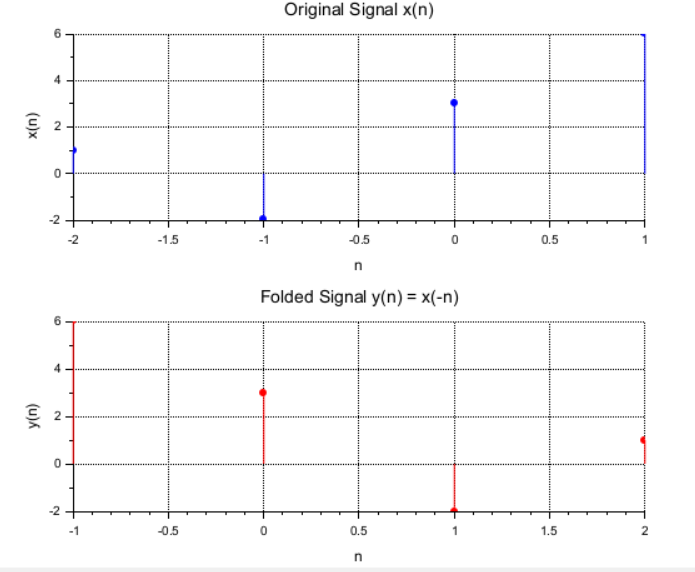
\includegraphics[width=0.65\textwidth]{img/ex3.png}
    \caption{Đồ thị tín hiệu gốc $x(n)$ và tín hiệu sau khi đảo $y(n) = x(-n)$}
\end{figure}

\noindent$\rightarrow$ \textbf{Nhận xét:} Tín hiệu $y(n)$ là ảnh đối xứng qua trục tung $n = 0$ của tín hiệu $x(n)$, mẫu tại gốc thời gian giữ nguyên giá trị ($y(0) = 3$).
